\setcounter{ExampleCounter}{1}
\subsection{Exponent Notation}

%We've used exponents a few times already in this chapter, but here we'll spend a bit more time focusing on them.\\

Exponent notation is simply a concise way to write down repeated multiplication.  This is particularly useful for some kinds of growth models.  For instance, suppose that some quantity starts at 100 and doubles every year.  The process would like something like this:
\begin{center}
\begin{tabular}{l r}
At beginning: & 100\\
After 1 year: & 100(2) = 200\\
After 2 years: & 100(2)(2) = 400\\
After 3 years: & 100(2)(2)(2) = 800\\
$\vdots$ & $\vdots$\\
After $t$ years: & $100 \left(2^t\right)$
\end{tabular}
\end{center}

Notice what this notation does for us: it simply saves us from having to write $(2)(2)\ldots (2)$ over and over and over again.

\begin{proc}{Exponent Notation}
Exponent notation represents repeated multiplication.  The \textbf{power} or \textbf{exponent} (the superscript) gives the number of times that the given quantity is multiplied by itself.\\

Ex: $3^4 = 3 \cdot 3 \cdot 3 \cdot 3 = 81$\\

Ex: $3^1 = 3$
\end{proc}

\begin{example}{Exponent Notation}
Evaluate the following exponential expression.
\[3 \cdot 2^3\]

\sol
\[3 \cdot 2^3 = 3 \cdot 2 \cdot 2 \cdot 2 = \boxed{8}\]
Notice that the exponent \emph{only} acts on the 2.
\end{example}

\begin{example}{Exponent Notation}
Evaluate the following exponential expressions.
\begin{enumerate}[(a)]
\item $-4^2$
\item $(-4)^2$
\end{enumerate}

\sol
As seen in the previous example, an exponent \emph{only} acts on whatever is written directly before it.

\begin{enumerate}[(a)]
\item Thus, in the first example, only the 4 gets multiplied repeatedly; the negative sign will only appear once.
\[-4^2 = - 4 \cdot 4 = \boxed{-16}\]
\item In the second example, though, the parentheses act (as they always do) to group together the negative sign with the 4, so that the exponent acts on \emph{both} of them (since the parenthesis group is what comes directly before the exponent, that is what the exponent acts on).
\[(-4)^2 = (-4)(-4) = \boxed{16}\]
\end{enumerate}
\end{example}

\begin{example}{Exponent Notation}
Evaluate the following exponential expression.
\[4(2-5)^3\]

\sol
Recall the order of operations: we first need to simplify everything inside the parentheses, then evaluate the exponential part, and finally carry out the multiplication.
\[4(2-5)^3 = 4(-3)^3 = 4(-27) = \boxed{-108}\]
\end{example}

\begin{proc}{Using Your Calculator}
Of course, rather than evaluating exponents manually, you can use your calculator to do this process for you.  To do so, use the $\boxed{\wedge}$ key to enter an exponent, using parentheses for grouping as necessary.
\begin{center}
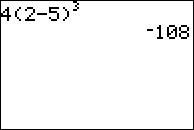
\includegraphics[height=1in]{Screen5}
\end{center}
\end{proc}

\subsection{Exponential Equations}

An exponential equation is one like the example given in the introduction: \[A = 100\left(2^t\right)\]

First, we need to note how this is different from the kinds of examples we did in the previous section, solving equations with powers.  The difference between the two kinds of examples is where the variable is:
\begin{center}
\begin{tabular}{c c}
\textbf{Power Equation} & \textbf{Exponential Equation}\\
\hline
\\
$x^2 = 16$ & $4^x = 16$\\ \\
Variable in the base & Variable in the exponent\\
Solve by taking the square root of both sides & Haven't shown how to solve yet
\end{tabular}
\end{center}

This distinction is important to understand, because when solving equations, we need to know what method to use.

\paragraph{Solving Exponential Equations} There are some exponential equations that can be solved just by using familiarity with common powers of small numbers.

\begin{example}{Solving Exponential Equations}
Solve for $x$: \[4^x = 16\]

\sol
By recognizing that 16 is a power of 4, we can spot the answer to this one:
\[4^x = 16 = 4^2 \longrightarrow \boxed{x = 2}\]
\end{example}

There are a few variations on this kind of problem, but ultimately, the most powerful tool for solving exponential equations is the \textbf{logarithm}.
\pagebreak

\subsection{Logarithms}

There are several common uses for logarithms, but the one that we will use elsewhere in this textbook is solving exponential equations that can't be solved as easily as the previous example (very few exponential equations can be solved that simply).\\

Just like a square root undoes a power of 2, a cube root undoes a power of 3, and so on, a logarithm undoes any exponent.  Here's the definition of a logarithm:
\[\textrm{If } y = a^x \textrm{, then } \log_a y = x.\]

This looks complicated, but if you look closely, you can see that it is simply a way of rearranging the pieces of an exponential equation in such a way that the exponent gets isolated (which is what we want when we solve an equation).  Since our calculators can calculate logarithms, we can use this definition to solve any exponential equation.

By the way, $\log_a y$ is read ``log base $a$ of $y$.''  The number $a$ is the \textbf{base} of the logarithm since it's the base of the exponent.

\begin{example}{Solving Exponential Equations Using Logarithms}
Solve the following equation for $x$ using logarithms:
\[4^x = 16\]

\sol
Of course, we already know the answer to this one since we solved it earlier, but we can illustrate how to use logarithms as well to get the same answer.\\

We simply need to apply the definition: to change this exponential equation into its equivalent logarithmic form, move the base of the exponent (4) to the other side of the equation as the base of the logarithm.  As it moves, the $x$ drops down from the exponent:
\[4^x = 16 \iff x = \log_4 16\]

Using a graphing calculator (as shown after the end of this example), we can calculate this answer:
\begin{center}
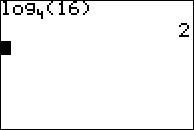
\includegraphics[scale=0.85]{Screen7}
\end{center}
\end{example}

\begin{proc}{Using Your Calculator}
To enter an expression like the one in the example above into a TI-84 calculator, locate the \verb|logBASE| function in the \verb|MATH| menu:
\begin{center}
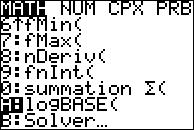
\includegraphics[scale=0.85]{Screen6}
\end{center}
This will place a logarithm on the screen with blanks in the base and inside the parentheses.\\

If your calculator does not have this function built in (or you cannot locate it; most calculators do have it somewhere), you can use what is known as the \textbf{change-of-base formula} with the \verb|LOG| key on your calculator.\\

To evaluate $\log_4 16$, for instance, using the change-of-base formula, you would type in \verb|log(16)/log(4)|.
\begin{center}
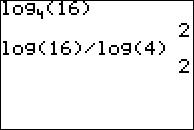
\includegraphics[scale=0.85]{Screen8}
\end{center}
\end{proc}

\begin{example}{Solving Exponential Equations Using Logarithms}
Solve the following exponential equation using logarithms:
\[2^x = 18\]

\sol
We can immediately rewrite this equation in logarithmic form by moving the 2 to the other side as the base of a logarithm:
\[2^x = 18 \iff x = \log_2 18 \approx \boxed{4.1699}\]

We could check this answer by raising 2 to the power of 4.17 (using a calculator of course).  Naturally, our answer wouldn't be exactly 18, since we rounded the exponent to 4.17, but it would be close enough to confirm our answer.
\end{example}
\pagebreak

\begin{example}{Solving Exponential Equations Using Logarithms}
Solve the following exponential equation using logarithms:
\[3^{2x-1} = 5\]

\sol
Again, we can use a logarithm to isolate what is currently in the exponent:
\[3^(2x-1) = 5 \iff 2x-1 = \log_3 5\]
Then, after calculating $\log_3 5$, we can solve this equation like any other linear equation: add 1 to both sides, then divide both sides by 2.
\begin{align*}
2x-1 &= \log_3 5 = 1.465\\
2x &= 2.465\\
x &= \dfrac{2.465}{2}\\ \\
x &= \boxed{1.232}
\end{align*}

This answer is also rounded, but correct to the level of precision that we need.
\end{example}

\begin{example}{Solving Exponential Equations Using Logarithms}
Solve the following exponential equation using logarithms:
\[100 = 25(1.005)^x\]

\sol
Here, before we change the equation into logarithmic form, we first need to isolate the exponential piece so that this equation looks like the others that we've solved.  Thus, divide both sides by 15 before applying the logarithm:
\begin{align*}
1.005^x &= \dfrac{100}{25} = 4\\
x &= \log_{1.005} 4\\ \\
x &= \boxed{277.95}
\end{align*}
\end{example}

\begin{example}{Solving Exponential Equations Using Logarithms}
Solve the following exponential equation using logarithms:
\[32 = \dfrac{6^x}{5}\]

\sol
Again, we need to isolate the exponential piece (by multiplying both sides by 5) before applying the logarithm:
\begin{align*}
32 &= \dfrac{6^x}{5}\\
(32)(5) = 160 &= 6^x\\
\log_6 160 &= x\\ \\
\boxed{2.833} &= x
\end{align*}
\end{example}

\begin{exercises}
\textit{In exercises 1--8, evaluate each exponential expression.}

\pfour{$2^4$}
\pfour{$-2^4$}
\pfour{$(-2)^4$}
\pfour{$-(-2)^4$}

\pfour{$2 \cdot 3^4$}
\pfour{$3(4+1)^2$}
\pfour{$5(1-1)^3$}
\pfour{$6+3^2$}

\textit{In exercises 9--16, solve each exponential equation.}

\pfour{$2^{x-5}=8$}
\pfour{$5^{-x} = 25$}
\pfour{$3^x=14$}
\pfour{$5\left(2^{3x}\right)=8$}

\pfour{$\left(\dfrac{4}{3}\right)^{1-x}=5$}
\pfour{$0.3(4^{0.2x})=0.2$}
\pfour{$2^x=10$}
\pfour{$2^{-x}=1.5$}

\vspace*{0.25in}

{\color{blue!60!black} \rule{\textwidth}{3pt}}
\vspace*{0.25in}

\subsection{Answers}
\begin{tabularx}{\textwidth}{l l l l l l}
1. 16 & 2. $-16$ & 3. 16 & 4. $-16$ & 5. 162 & 6. 75\\ \\
7. 0 & 8. 15 & 9. $x=8$ & 10. $x=-2$ & 11. $x \approx 2.4$ & 12. $x \approx 0.226$\\ \\
13. $x \approx -4.59$ & 14. $x \approx -1.46$ & 15. $x \approx 3.32$ & 16. $x \approx -0.585$
\end{tabularx}
\end{exercises}











